\chapter{Trabajo Relacionado}
\label{cap:trabajoRelacionado}

En este capítulo se revisan trabajos y enfoques relacionados con los principales módulos del sistema desarrollado. Dado que el proyecto combina varias áreas, el análisis no se limita a una única línea de investigación, sino que se organiza según las fases más relevantes del pipeline: detección de jugadores y balón, tracking multiobjeto y detección de eventos futbolísticos.

El objetivo de esta revisión es contextualizar las decisiones técnicas adoptadas en el proyecto, identificar alternativas existentes y señalar las principales dificultades asociadas a cada tarea. De este modo, el capítulo sirve como puente entre las tecnologías introducidas previamente y la descripción concreta del sistema implementado.


\section{Detección de jugadores y balón en fútbol}

La detección de objetos es una de las primeras fases necesarias para cualquier sistema automático de análisis de fútbol, ya que permite localizar en cada frame los elementos relevantes del juego, como jugadores, porteros, árbitros y balón.

Diversos trabajos han abordado este problema como una fase previa para tareas de análisis más complejas. \citet{KomorowskiFootAndBall2020} proponen FootAndBall, un detector conjunto de jugadores y balón orientado específicamente al dominio futbolístico. Este tipo de propuestas muestra que la detección del balón requiere una atención especial, al tratarse de un objeto pequeño, visualmente ambiguo y con frecuentes pérdidas de detección en cámaras broadcast.

Frente a YOLO, una alternativa clásica son los detectores de dos etapas, como Faster R-CNN. Este método propuesto por \citet{RenFasterRCNN2015} introduce una red de propuesta de regiones, o \textit{Region Proposal Network}, para generar zonas candidatas antes de clasificarlas y refinar sus cajas. Esta estrategia suele ofrecer detecciones precisas, pero implica un coste computacional mayor y una arquitectura menos directa para un pipeline de vídeo que debe ejecutarse frame a frame.

Otra alternativa reciente son los detectores basados en Transformers. DETR \citep{CarionDETR2020} introdujo una formulación de la detección como predicción directa de un conjunto de objetos, eliminando la necesidad de muchos componentes heurísticos habituales en detectores clásicos. Sobre esta línea, RF-DETR \citep{RobinsonRFDETR2026} plantea una variante orientada a detección en tiempo real, buscando un compromiso entre precisión y latencia. Este tipo de modelos resulta interesante como alternativa moderna a YOLO, ya que las arquitecturas basadas en Transformers pueden capturar relaciones globales entre objetos y adaptarse bien a dominios nuevos.

En este proyecto se opta por YOLO, descrito con más detalle en la \hyperref[sec:yolo-tecnologias]{Sección~\ref*{sec:yolo-tecnologias}}, por su madurez práctica, disponibilidad de herramientas de \textit{fine-tuning}, integración sencilla con el resto del pipeline y buen equilibrio entre velocidad y precisión en vídeo.
\section{Tracking multiobjeto en vídeo deportivo}

El tracking multiobjeto es una tarea especialmente compleja en fútbol debido a las oclusiones, los cruces entre jugadores, la similitud visual entre compañeros de equipo, los cambios de cámara y las detecciones intermitentes. Estas dificultades han motivado el uso de distintos enfoques de asociación temporal y reidentificación para mantener identidades consistentes a lo largo del vídeo.

Una alternativa habitual es DeepSORT, propuesto por \citet{WojkeDeepSORT2017}, que extiende SORT incorporando descriptores de apariencia aprendidos mediante redes de reidentificación. Además de la predicción de movimiento mediante el filtro de Kalman \citep{Kalman1960}, DeepSORT compara las detecciones con las trayectorias activas utilizando tanto información geométrica como apariencia visual. La \hyperref[fig:deepsort-esquema]{Figura~\ref*{fig:deepsort-esquema}} muestra un esquema general de este funcionamiento.

\begin{figure}[H]
    \centering
    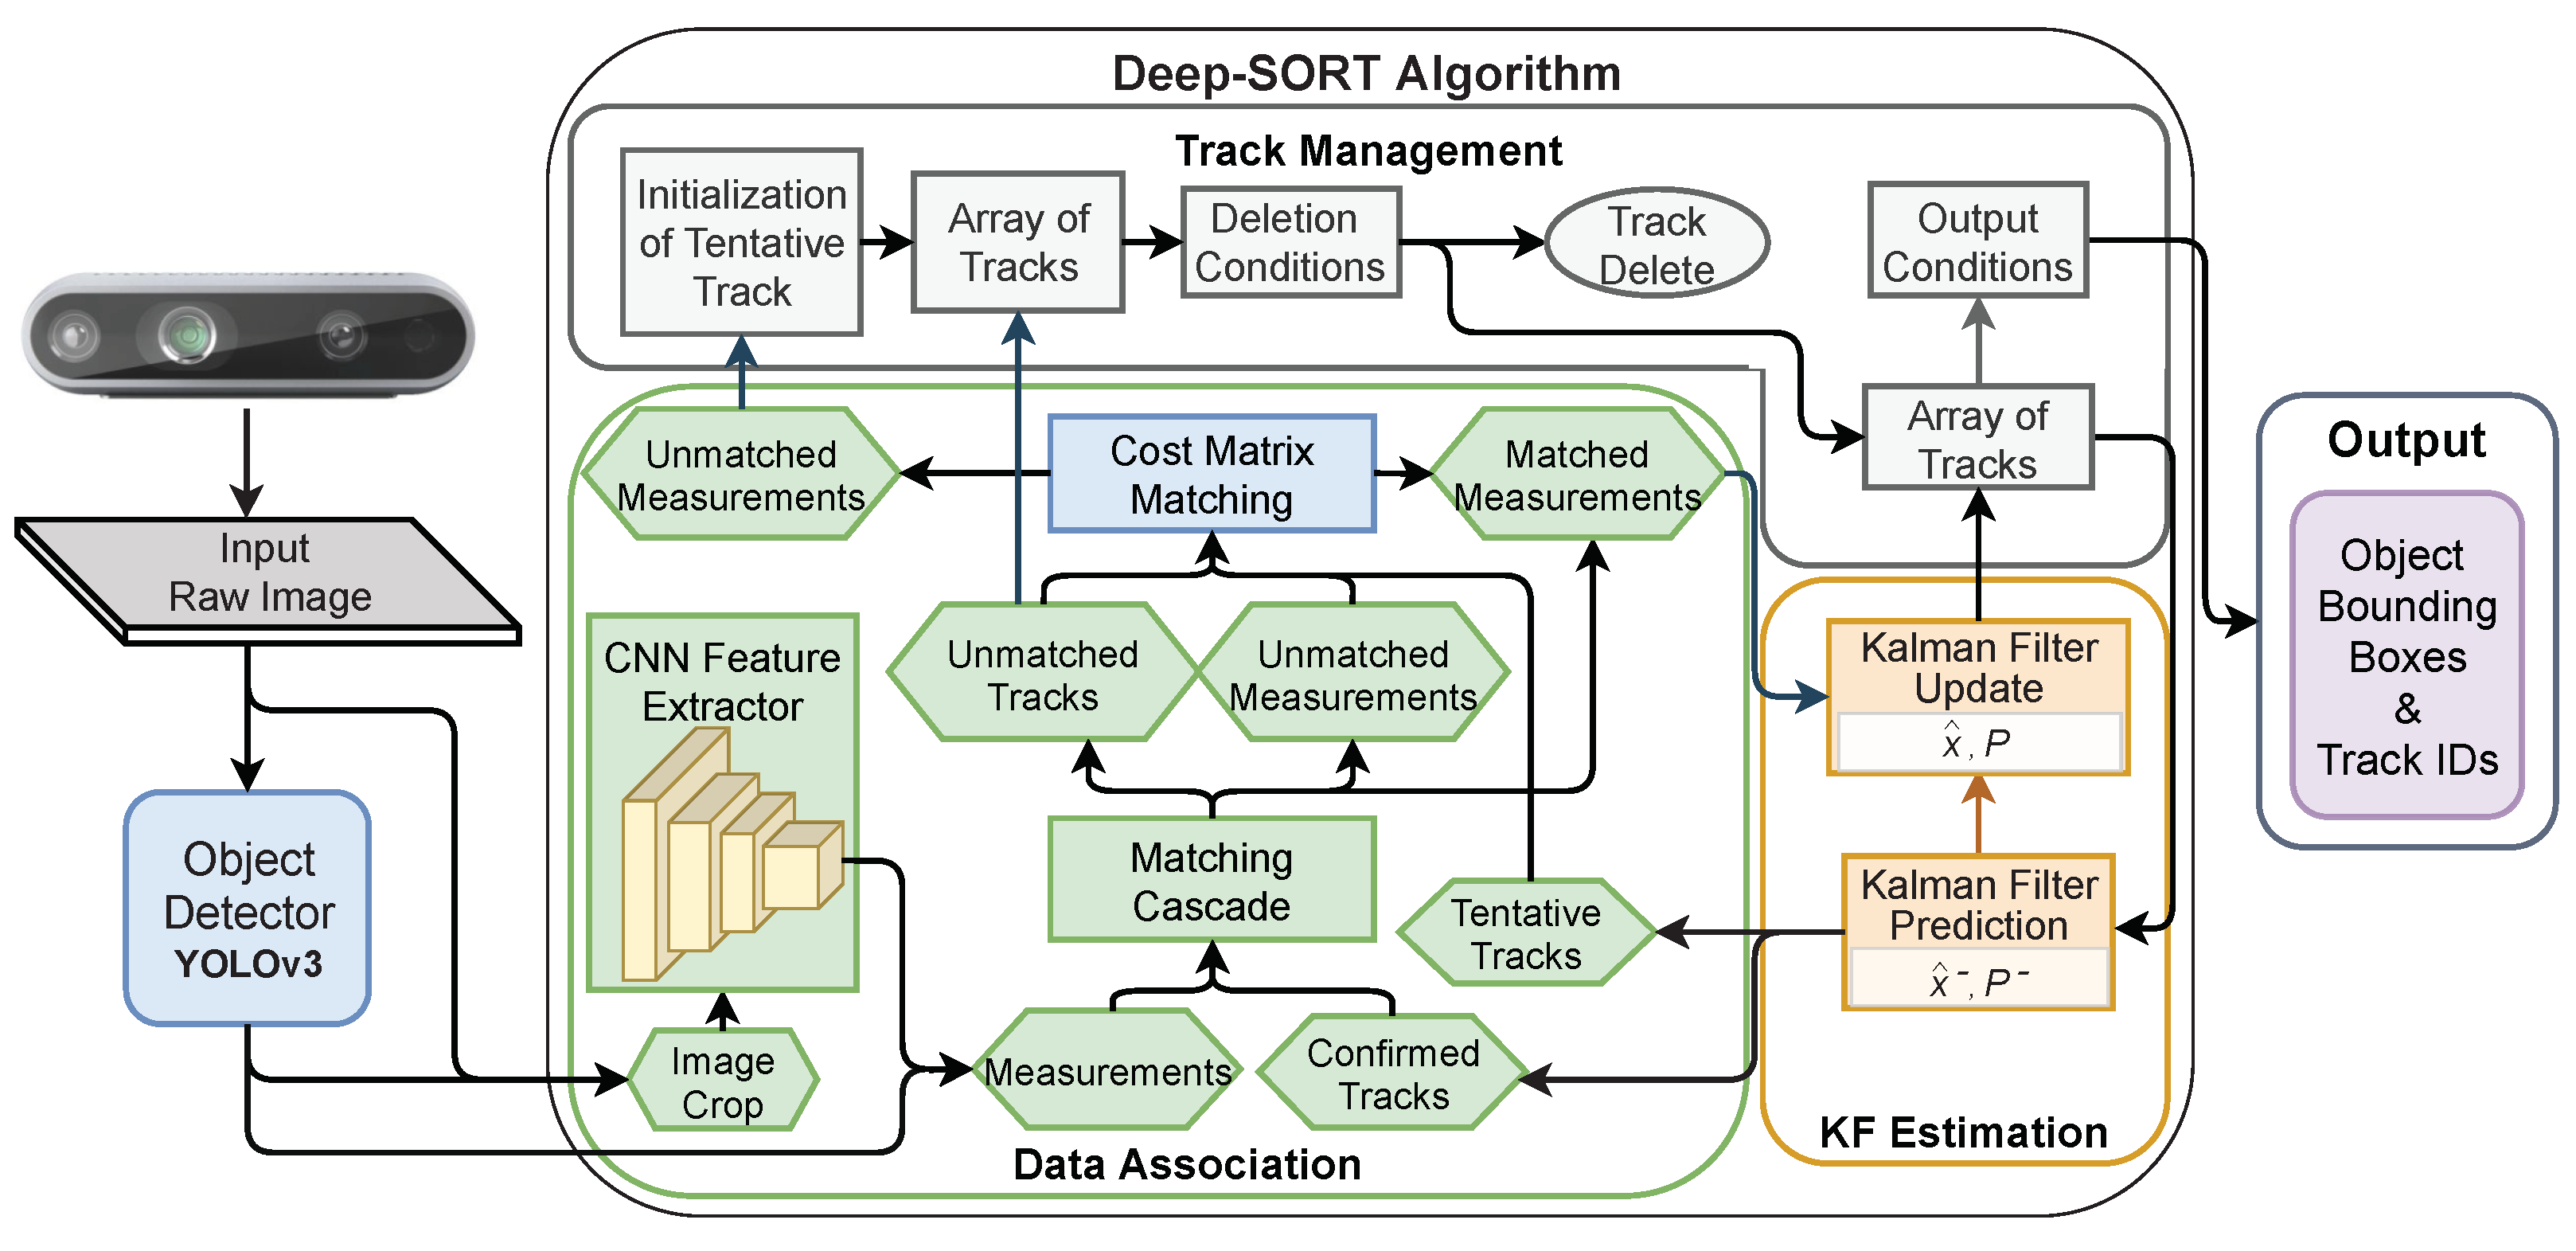
\includegraphics[width=0.9\textwidth]{Imagenes/Propias/DeepSort.png}
    \caption[Esquema general de DeepSORT]{
    Esquema general de DeepSORT. El método combina predicción mediante filtro de Kalman, asociación de detecciones y un descriptor de apariencia obtenido con una red convolucional, lo que ayuda a mantener identidades cuando el movimiento por sí solo no basta. Fuente: reproducido de \citep{PereiraDeepSORT2022}.
    }
    \label{fig:deepsort-esquema}
\end{figure}

Este enfoque puede reducir cambios de identidad en escenarios donde la apariencia visual ayuda a distinguir personas, como vigilancia o seguimiento de peatones. Sin embargo, en fútbol broadcast la apariencia puede ser menos discriminativa, ya que muchos jugadores del mismo equipo llevan equipaciones casi idénticas y las cajas pueden tener baja resolución. Además, entrenar o utilizar descriptores de reidentificación robustos para jugadores concretos requiere datos adicionales que no siempre están disponibles.

Otra alternativa relevante es OC-SORT, propuesto por \citet{CaoOCSORT2023}. Este método revisa el uso del filtro de Kalman en tracking y plantea una asociación más centrada en las observaciones reales, reduciendo errores acumulados durante oclusiones o movimientos no lineales. Este enfoque resulta interesante para deportes, ya que los jugadores no siempre siguen trayectorias suaves y pueden realizar cambios bruscos de dirección.

Frente a estas alternativas, ByteTrack resulta atractivo para sistemas de análisis deportivo por su equilibrio entre simplicidad, eficiencia y robustez ante detecciones de baja confianza. Su enfoque permite recuperar objetos que un tracker convencional podría descartar prematuramente, algo especialmente útil en escenas con oclusiones, agrupaciones de jugadores o detecciones inestables.
\section{Detección de eventos en fútbol}

La detección de eventos en fútbol tiene como objetivo identificar cuándo ocurren acciones relevantes del partido y asignarles una interpretación semántica, como pase, tiro, falta, saque o cambio de posesión. Esta tarea es especialmente compleja porque muchas acciones no pueden reconocerse únicamente a partir de un único frame, sino que dependen de la evolución temporal de jugadores, balón y contexto de juego.

Una línea de trabajo relacionada es el \textit{action spotting}, cuyo objetivo consiste en localizar temporalmente acciones relevantes dentro de vídeos largos de partido. En fútbol, SoccerNet \citep{GiancolaSoccerNet2018} ha sido una de las principales referencias para esta tarea, al proporcionar un amplio dataset de partidos broadcast con anotaciones temporales de eventos. Posteriormente, SoccerNet-v2 \citep{DeliegeSoccerNetV22021} amplió el dataset con anotaciones más densas y nuevas tareas de comprensión de vídeo, incluyendo acciones, cambios de cámara y repeticiones.

En vídeo broadcast, muchos trabajos abordan la detección de acciones directamente a partir de la señal visual. Una línea clásica consiste en combinar extractores convolucionales con modelos temporales: primero se obtiene una representación visual de cada frame mediante una CNN y después se modela la evolución temporal de la secuencia con redes recurrentes o LSTM, como en LRCN \citep{DonahueLRCN2015}. Otra línea emplea arquitecturas espaciotemporales, como I3D \citep{CarreiraI3D2017}, capaces de capturar conjuntamente apariencia y movimiento a partir de convoluciones 3D. Estos enfoques son potentes, pero suelen requerir grandes cantidades de vídeo anotado, diversidad visual y un coste computacional considerable.

Dentro del contexto de SoccerNet, se han propuesto métodos específicos para \textit{action spotting} en fútbol broadcast. \citet{CioppaCALF2020} introducen CALF, una función de pérdida consciente del contexto temporal que permite localizar acciones alrededor de un instante anotado, evitando tratar cada frame de forma completamente aislada. Posteriormente, NetVLAD++ \citep{GiancolaNetVLAD2021} propone una agregación temporal que separa el contexto anterior y posterior a una acción, mejorando la representación de eventos en secuencias largas. Más recientemente, T-DEED \citep{XarlesTDEED2024} busca aumentar la resolución y discriminabilidad temporal de las predicciones para eventos deportivos. Este tipo de métodos resulta especialmente relevante para tareas como BAS (\textit{Ball Action Spotting}), donde se pretende detectar acciones relacionadas con el balón directamente desde el vídeo.

Frente a los enfoques basados principalmente en frames RGB, PathCRF \citep{KimPathCRF2026} plantea una alternativa basada en trayectorias estructuradas de jugadores. Como se describe con más detalle en la \hyperref[sec:pathcrf-tecnologias]{Sección~\ref*{sec:pathcrf-tecnologias}}, el modelo infiere una secuencia de estados de posesión y extrae eventos a partir de sus cambios. Su entrenamiento y evaluación se apoyan en el \textit{Sportec Open DFL Dataset}, publicado por \citet{BassekIntegratedDataset2025}, que proporciona eventos anotados y datos posicionales oficiales de partidos de la Bundesliga.

En resumen, métodos como LRCN, I3D, CALF, NetVLAD++ o T-DEED representan enfoques consolidados para detectar eventos desde vídeo broadcast. Sin embargo, PathCRF resulta especialmente interesante para pipelines que ya construyen una representación geométrica y temporal del partido, ya que permite transformar trayectorias de jugadores en eventos semánticos utilizables por etapas posteriores.